\documentclass[10pt,letterpaper]{article}
\usepackage[margin=0.82in]{geometry}
\usepackage[T1]{fontenc}
\usepackage{lmodern,amsmath,amssymb,booktabs,graphicx,xcolor,hyperref,fancyhdr}
\usepackage{microtype}
\definecolor{navy}{HTML}{153A52}
\definecolor{teal}{HTML}{007F82}
\hypersetup{colorlinks=true,linkcolor=navy,citecolor=teal,urlcolor=teal,pdftitle={Classical Search in Chess},pdfauthor={Akbar Aman}}
\pagestyle{fancy}\fancyhf{}\fancyhead[L]{\small MURL \;|\; Experiment 01}\fancyhead[R]{\small Classical chess search}\fancyfoot[C]{\thepage}
\setlength{\headheight}{14pt}\setlength{\parindent}{0pt}\setlength{\parskip}{4pt}
\newcommand{\talk}[1]{\par\smallskip\noindent{\color{teal}\textbf{Meeting takeaway.}} #1\par}
\newcommand{\code}[1]{\texttt{\detokenize{#1}}}
\newcommand{\RunCount}{144}

\begin{document}
\thispagestyle{empty}
{\color{teal}\small UIC MATH 496 \quad MACHINE LEARNING, CHESS AND MATHEMATICS}
\vspace{0.25in}

{\color{navy}\LARGE\bfseries Classical Search in Chess\par}
\vspace{0.06in}
{\large An Empirical Comparison of MinMax and Monte Carlo Tree Search in Python\par}
\vspace{0.15in}
\textbf{Akbar Aman}\hfill September 23, 2026\par
Prepared for the 8:30 PM meeting with Evangelos Kobotis and Drew Shulman.

\section{Objective and research question}
The assignment asks for Python implementations of MinMax and Monte Carlo Tree Search (MCTS), using \code{python-chess}, and an experiment on positions with different amounts of material. The question here is operational: \emph{At which tested depths and simulation budgets can these straightforward implementations return a move within an interactive time allowance?}

This is a computational baseline, not a chess-strength contest. Eight positions span four to thirty-two pieces. Equal-material pairs help separate piece count from mobility. The experiment records legal moves, tree nodes, elapsed time, selected moves, completion status, and MCTS rollout statistics. All tables and figures are generated from actual executions; no engine evaluations or estimated runtimes are substituted for measurements.

\subsection*{What to listen for}
\begin{itemize}
\item \textbf{Material describes the board; branching describes the search.} Pieces constrain available moves, but their type and arrangement matter too.
\item \textbf{Depth multiplies work.} Looking one move farther means exploring replies below many existing positions.
\item \textbf{A simulation budget controls MCTS effort, not move quality.} Returning quickly does not establish that a move is strong.
\end{itemize}

\section{Background: a tree of possible futures}
A chess position is a state; each legal move is an edge to a successor state. A \emph{ply} is one player's move. Searching to depth three therefore examines our move, the opponent's reply, and our next move. A full game tree is far too large for this experiment, so both algorithms stop early and use a simple evaluation.

Shannon's foundational chess-programming paper connects game-tree search with position evaluation~\cite{shannon1950}. Modern textbook adversarial search supplies the MinMax and cutoff framework~\cite{aima2021}. Our implementation follows the alternating MAX/MIN structure of the official AIMA companion pseudocode, explicitly labeled third edition~\cite{aimaPseudocode}. MCTS follows the four-stage organization in Browne et al., with UCT selection from Kocsis and Szepesv\'ari~\cite{browne2012,kocsis2006}. These are conceptual adaptations; no tutorial or engine implementation was copied.

\talk{I treated the assignment as a small research study: build transparent algorithms, control the workloads, and ask what the timings actually justify.}

\newpage
\section{MinMax: assume the opponent chooses well}
Let $s$ be a position, $A(s)$ its legal moves, and $s_a$ the position after move $a$. All values favor White when positive. With $d$ plies remaining,
\[
V(s,d)=\begin{cases}
U(s),&s\text{ is terminal},\\
E(s),&d=0,\\
\max_{a\in A(s)}V(s_a,d-1),&\text{White to move},\\
\min_{a\in A(s)}V(s_a,d-1),&\text{Black to move}.
\end{cases}
\]
In plain English, White chooses the largest available score and Black chooses the smallest. The algorithm works backward from the evaluated leaves. It does not assume the opponent cooperates. At the root it returns the legal move attaining the appropriate maximum or minimum.

\subsection{What the evaluation measures}
\[
E(s)=\sum_{p\in\{P,N,B,R,Q\}} w_p\bigl(n_{W,p}(s)-n_{B,p}(s)\bigr),
\qquad (w_P,w_N,w_B,w_R,w_Q)=(1,3,3,5,9).
\]
Here $n_{W,p}$ and $n_{B,p}$ count White's and Black's pieces of type $p$. A score of $+3$ means White has three more weighted pawn units of material. Kings contribute zero material points because both sides retain a king in a valid position. Checkmate overrides material: $U=+10{,}000$ for a White win, $-10{,}000$ for a Black win, and zero for a draw. The large mate value makes any detected win preferable to material gain. It does not reward faster mates.

Material is easy to audit, but ignores king safety, pawn structure, development and positional compensation. In a quiet opening, many moves tie. The first tied legal move in the library's enumeration wins the tie; that is a deterministic implementation choice, not a claim of chess merit.

\subsection{Why depth is expensive}
If every internal node has roughly $b>1$ children, the number of visited nodes is
\[
N(d)\approx 1+b+b^2+\cdots+b^d=\frac{b^{d+1}-1}{b-1}=O(b^d).
\]
Thus an extra ply can multiply work by approximately $b$, rather than add a fixed amount. If average node cost is $c$, wall time is approximately $cN(d)$. Real chess has variable branching, terminal branches, and unequal node costs, so root legal-move count is only a proxy for the deeper tree. Ratios $N(d)/N(d-1)$ are empirical growth factors, not a universal chess constant.

The implementation deliberately uses \textbf{plain MinMax}: no alpha-beta pruning, transposition table, ordering heuristic, quiescence search, or iterative deepening. Alpha-beta is a natural next controlled extension: with the same leaves and evaluation it can preserve the MinMax value while skipping branches that cannot affect the decision~\cite{aima2021}. It is not included in the reported benchmark.

\talk{MinMax asks, ``What is my best outcome if the opponent always picks the reply that is worst for me?'' Its answer is exact for the truncated tree and evaluator, not for the full game.}

\newpage
\section{MCTS: spend simulations selectively}
MCTS grows a partial tree through repeated simulations instead of exhaustively traversing a fixed depth. One iteration has four stages~\cite{browne2012}:
\begin{enumerate}
\item \textbf{Selection:} follow existing tree edges using the UCT rule below.
\item \textbf{Expansion:} add one uniformly selected untried legal move when available.
\item \textbf{Simulation:} play uniformly random legal moves until a terminal outcome or a forty-ply rollout limit.
\item \textbf{Backpropagation:} add the resulting reward and one visit to every node on the selected path.
\end{enumerate}

\subsection{The exploration--exploitation balance}
For a parent $v$ and visited child $i$, selection maximizes
\[
\operatorname{UCT}(v,i)=q(v,i)+\sqrt{2}\sqrt{\frac{\ln N_v}{N_i}},\qquad
q(v,i)=\begin{cases}\bar r_i,&\text{White at }v,\\1-\bar r_i,&\text{Black at }v.\end{cases}
\]
$N_v$ and $N_i$ are visit counts, and $\bar r_i$ is the child's average White reward. The first term favors moves with good observed outcomes (\emph{exploitation}). The second favors relatively underexplored moves (\emph{exploration}). As a child receives more visits, its exploration bonus falls; as the parent is revisited, neglected children become more attractive. Untried moves are expanded before this competition; an unvisited child receives infinite priority.

All stored rewards use White's perspective. At a Black parent, replacing $\bar r$ by $1-\bar r$ makes Black prefer outcomes favorable to Black. Without that change, the tree policy would model a cooperating opponent. The same White reward can then be propagated unchanged through all ancestors. The chosen exploration constant is a conventional baseline setting, not a tuned optimum~\cite{kocsis2006}.

\subsection{What a rollout reward means}
A White win gives reward $1$, a draw $1/2$, and a Black win $0$. Most short rollouts need not finish a game. At the forty-ply cap, the code uses
\[
r(s)=\tfrac12\left[1+\tanh\left(E(s)/10\right)\right].
\]
The hyperbolic tangent smoothly compresses material advantage into a bounded scale: equal material maps to $1/2$, positive material above $1/2$, and negative material below it. The ten-pawn divisor controls sensitivity. It is declared in advance, not fitted to these results. \textbf{This is a heuristic utility, not a calibrated probability of winning.} The forty-ply cap applies after the selected tree path, not to total search depth.

The final decision is the most-visited root child (the ``robust child'' rule), with ties broken by the mover's mean reward and then seeded expansion order~\cite{browne2012}. The code records every root move's visits and mean reward. A fixed iteration budget bounds simulation count, but each iteration costs different time because move generation, rollout length, terminal detection and tree depth vary.

\talk{MinMax systematically backs up worst-case replies. MCTS samples futures and allocates more attention to promising or insufficiently explored choices. Random rollouts can miss a single decisive tactical refutation.}

\newpage
\section{Experimental method}
\subsection{Rules, positions and controlled choices}
\code{python-chess} handles FEN parsing, legal moves, board copies, move application and reversal, and standard terminal detection~\cite{pythonChess}. A FEN is a compact text description of a board plus side to move and rule state. Every fixture must pass \code{Board.is_valid()}, have its expected material count, and be nonterminal before timing. Validity checks do not prove historical reachability.

\begin{center}\small
\begin{tabular}{llrr}
\toprule
ID & Position & Pieces & Root moves \\
\midrule
R4 & Four-piece rook ending & 4 & 21 \\
R7 & Seven-piece rook ending & 7 & 21 \\
R11 & Eleven-piece rook ending & 11 & 24 \\
P16 & Sixteen-piece pawn blockade & 16 & 15 \\
M16 & Sixteen-piece mixed position & 16 & 53 \\
M24 & Reduced middlegame & 24 & 42 \\
S32 & Initial position & 32 & 20 \\
I32 & Italian development & 32 & 33 \\
\bottomrule
\end{tabular}
\end{center}


The first six positions are deliberately constructed controls. The final two are the initial position and the legal sequence 1.e4 e5 2.Nf3 Nc6 3.Bc4 Bc5. All are White to move. Equal-size pairs at sixteen and thirty-two pieces make mobility contrasts visible; the suite is not a random sample of chess games. It was specified before inspecting timings.

Both searches handle checkmate, stalemate and library-detected automatic draws before evaluation. Optional threefold-repetition and fifty-move claims are not modeled as player actions (\code{claim_draw=False}). Automatic fivefold repetition and seventy-five-move draws are recognized when the available history permits. FEN does not supply prior repetition history. The library's documented insufficient-material detector does not solve every possible dead-position case~\cite{pythonChess}.

\subsection{Timing, environment and practical thresholds}
Measurements were made on September 23, 2026 (America/Chicago), using AMD Ryzen 7 7730U with Radeon Graphics, 16 logical CPUs available, Windows 11, CPython 3.12.14, \code{python-chess} 1.999 (\code{chess} 1.11.2). No CPU affinity or frequency control was applied; available logical CPUs do not mean the search was parallelized.

The algorithms run sequentially on one process. Wall-clock timing uses \code{time.perf_counter()} around the complete search call. It includes algorithm validity guards, internal copies, move generation, terminal checks and evaluation; it excludes imports, fixture preparation, warmup, output formatting and file writes. One short warmup per algorithm precedes the measurements. All conditions and repetitions are shuffled using schedule seed 20260923.

MinMax uses depths 1--4; MCTS uses 100 and 400 iterations with forty-ply rollouts. Three runs per condition produce \RunCount{} measured searches. MCTS repetition seeds are 0, 1 and 2, so its timing spread combines different sampled paths with system noise. Tables report medians; raw rows and min/max remain available. No confidence intervals or population inference are justified by three repeats.

For interpretation, the operational categories are: a median at most one second is \emph{interactive}; above one and at most five seconds is \emph{meeting-tolerable}; above five seconds is \emph{slow for live use}. Each call has a cooperative fifteen-second deadline. A timeout is incomplete, not a completed fifteen-second result. Mixed completion groups must not be interpreted using successful runs alone. These thresholds are descriptive study conventions, not preregistered hypotheses or definitions of acceptable chess-engine strength.

\newpage
\section{Measured results}
\begin{center}\small
\setlength{\tabcolsep}{7pt}
\begin{tabular}{lrrrrr}
\toprule
 & \multicolumn{3}{c}{MinMax depth} & \multicolumn{2}{c}{MCTS iterations} \\
\cmidrule(lr){2-4}\cmidrule(lr){5-6}
ID & 2 & 3 & 4 & 100 & 400 \\
\midrule
R4 & 0.017 & 0.217 & 4.017 & 0.196 & 0.878 \\
R7 & 0.013 & 0.281 & 5.096 & 0.210 & 0.839 \\
R11 & 0.012 & 0.227 & 3.647 & 0.213 & 0.860 \\
P16 & 0.007 & 0.087 & 1.098 & 0.195 & 1.110 \\
M16 & 0.076 & 3.586 & \textit{TO} & 0.265 & 1.580 \\
M24 & 0.067 & 1.756 & \textit{TO} & 0.315 & 1.142 \\
S32 & 0.015 & 0.268 & 6.194 & 0.267 & 1.596 \\
I32 & 0.035 & 1.141 & \textit{TO} & 0.418 & 1.265 \\
\bottomrule
\end{tabular}
\end{center}
{\small\textbf{Table 1.} Median elapsed seconds across three runs per condition. TO means all three searches reached the fifteen-second deadline before completing the requested depth. Timeout durations are censored observations, not full-depth runtimes. Depth-one results and all individual runs remain in the raw CSV.}

Of 144 calls, 135 completed and 9 reached the deadline; 0 execution errors were recorded. All nine timeouts occurred at depth four: all repetitions of the mixed sixteen-piece position, the twenty-four-piece middlegame, and the Italian position. Their full-depth runtimes are unknown.

The sixteen-piece pair is especially informative. The pawn position has 15 root moves and took 0.087 seconds at depth three; the mixed position has 53 and took 3.586 seconds, a 41.3-fold median difference. Their exact node counts are 2,978 and 123,342, a 41.4-fold workload difference.

The initial and Italian positions both have 32 pieces, but depth-three medians were 0.268 and 1.141 seconds. Initial-position depth four completed in 6.194 seconds; every Italian depth-four attempt timed out.


\begin{center}
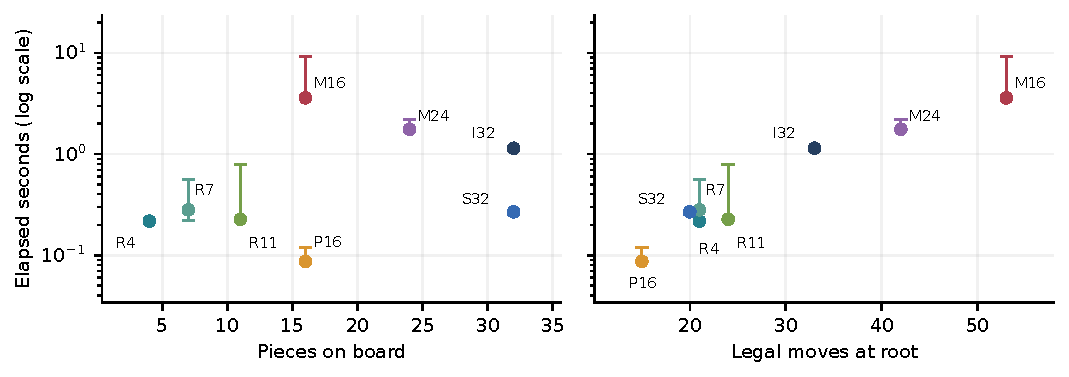
\includegraphics[width=\linewidth]{../results/figures/runtime_mobility.pdf}
\end{center}
{\small\textbf{Figure 1.} Depth-three MinMax runtime versus piece count and root legal moves. Points are position-level medians; bars show the observed minimum and maximum over three runs. Labels identify fixtures. The horizontal comparison is descriptive; it does not isolate a causal effect of adding pieces.}

\subsection{Material versus mobility}
Piece count is a useful experimental variable, but it does not uniquely specify the number of legal moves or the deeper reply tree. A rook on an open board can move along many squares; a pawn may have only a few options or be blocked. Even identical root mobility can lead to different reply counts, captures and terminal states. The paired positions are evidence for this distinction, not proof that root legal moves perfectly predict time.

\talk{The practical question is not ``How many pieces can Python handle?'' It is ``Which position, which depth or budget, with which implementation and time allowance?''}

\newpage
\section{Interpreting depth and simulation budgets}
\begin{center}
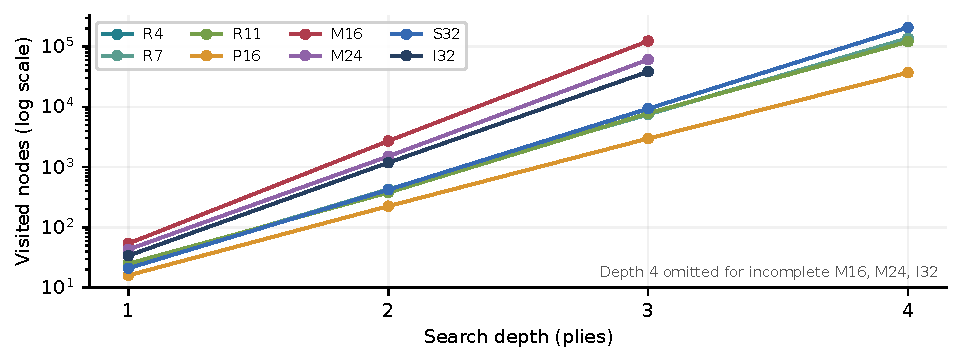
\includegraphics[width=0.88\linewidth]{../results/figures/node_growth.pdf}
\end{center}
{\small\textbf{Figure 2.} MinMax visited nodes versus depth, on a logarithmic vertical scale. Only fully completed depth conditions appear as ordinary points. A missing censored depth must not be extrapolated into a measured full tree. The count includes the root and every entered recursive node.}

\begin{center}
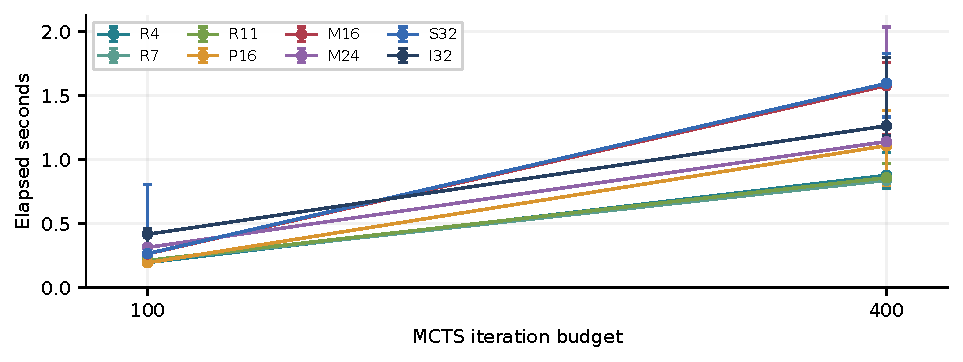
\includegraphics[width=0.88\linewidth]{../results/figures/mcts_budget.pdf}
\end{center}
{\small\textbf{Figure 3.} MCTS runtime at two iteration budgets; medians with observed min/max. More iterations mean more simulations, but do not impose an identical workload across positions or guarantee better choices in any particular run.}

For the initial position, MinMax visited 21, 421, 9,323, and 206,604 nodes at depths one through four. The last step multiplied nodes by 22.16 and median runtime by 23.12. This is the practical consequence of an expanding reply tree.

Increasing MCTS from 100 to 400 iterations multiplied median time by between 3.03 and 5.99 across these positions. Approximately linear budget scaling is a useful expectation, not an exact law from two points. Across all MCTS calls, 11,653 of 12,000 simulations (97.1\%) stopped at the rollout cap, showing how strongly this experiment depends on heuristic evaluation.

Timing variation was substantial in some conditions: mixed-position depth three ranged from 3.528 to 9.261 seconds despite identical node counts. System load or frequency variation is a plausible explanation, not a measured diagnosis. Medians reduce sensitivity to a single slow run; the ranges remain part of the evidence.

MinMax's node count measures evaluated and expanded search positions. MCTS's stored-tree node count excludes the many rollout positions. Comparing those two node counts directly as equal units of computational work would be misleading. Likewise, a MinMax pawn score and an MCTS bounded reward do not share a numeric scale.

\newpage
\section{Computational limits and engine context}
\subsection{What these measurements establish}
Across the 48 position--budget conditions, 32 had completed-run medians at most one second, 11 were between one and five seconds, and 2 exceeded five seconds with all repetitions complete. Three additional conditions timed out on all repetitions. All tested depth-three conditions completed, but that does not make all of them interactive. At depth four, only five of eight positions completed within the deadline in all three trials. All MCTS budgets completed; four hundred simulations remain a small sample of chess continuations.

These are feasibility statements about this program on this machine. A quick answer may be tactically poor, and a slow search may still use a weak evaluator. The experiments do not measure win rate, best-move accuracy, Elo, or an equal-strength speed comparison. They support the narrower conclusion: \emph{straightforward Python search becomes computationally expensive as branching and depth increase.}

Python's interpreter, loops, objects and library calls add runtime overhead. Move generation, terminal checks and history copying also cost time. This whole-program benchmark does not isolate these components or a language-only overhead factor; time per node also reflects machine state.

\subsection{Why Stockfish is a different comparison}
The instructors' C++ comparison motivates care, not a direct benchmark claim. As a pinned example, official Stockfish 17.1 source combines compiled C++ with alpha-beta search and cutoffs, selective pruning, move ordering, transposition tables, quiescence search and NNUE evaluation~\cite{stockfish2025}. A transposition table reuses information when different move sequences reach the same position. Move ordering brings likely useful moves forward so cutoffs become more effective. NNUE supplies learned evaluation within a heavily engineered search system.

Consequently, language, search policy, data structures and evaluation all differ. Stockfish was not run here. No Python-to-C++ speed ratio, engine ranking, or claim that ``MinMax is unusable for chess'' follows from this study.

\section{Limitations and next research step}
Eight hand-selected positions, one computer, three repetitions, shallow depths and short simulations cannot represent chess as a whole. Runtime can change with background load, power management and temperature. The evaluator has a horizon effect: consequences just beyond the cutoff are unseen. Random rollouts are strategically weak, and the material transform introduces a deliberate heuristic bias. All fixtures use White to move, although correctness tests exercise Black's perspective. Dead-position detection and optional draw claims have the limits described earlier.

The next controlled search experiment is alpha-beta with the same evaluator and positions, checking value agreement with plain MinMax. Later, a stronger evaluator could be assessed under matched wall-clock budgets. Akbar's longer-term direction is
\[
\begin{gathered}
\text{Classical search}\longrightarrow\text{observed computational limits}\\
\longrightarrow\text{stronger evaluation}\longrightarrow\text{Stockfish-supervised data}\\
\longrightarrow\text{learned evaluation combined with search}.
\end{gathered}
\]
Those engine-labeling and machine-learning stages are proposed work, not completed results. Better evaluation is a hypothesis to test against held-out positions and a fixed computation budget, not a substitute for legality or adversarial reasoning.

\section{Conclusion}
Two inspectable algorithms and reproducible measurements establish a baseline: material alone is insufficient; depth and branching matter strongly; MCTS offers a different budget--quality tradeoff. This supports controlled search improvements before introducing learned evaluation.

\newpage
\appendix
\section{Positions and reproducibility}
The exact FENs below include side to move, castling rights, en-passant state and move counters. They are also stored in \code{experiments/search_baseline/positions.py}.
\begingroup\footnotesize
\textbf{R4: rook\_04}\\
\texttt{8/5k2/6r1/8/8/1R6/2K5/8 w - - 0 1}\par\smallskip
\textbf{R7: rook\_pawns\_07}\\
\texttt{8/5pk1/6p1/8/2P5/2K5/1R6/6r1 w - - 0 1}\par\smallskip
\textbf{R11: rook\_pawns\_11}\\
\texttt{8/4rpk1/5pp1/8/2P1P3/P1K2P2/1R6/8 w - - 0 1}\par\smallskip
\textbf{P16: pawns\_16}\\
\texttt{6k1/8/8/pppppp1p/PPPPPP1P/8/8/6K1 w - - 0 1}\par\smallskip
\textbf{M16: mixed\_16}\\
\texttt{r3k3/1p2bpp1/2n5/3q4/3Q4/2N5/1P2BPP1/R3K3 w - - 0 1}\par\smallskip
\textbf{M24: middlegame\_24}\\
\texttt{r2q1rk1/ppp2ppp/2nb4/8/3P4/2NB4/PP3PPP/R2Q1RK1 w - - 0 1}\par\smallskip
\textbf{S32: initial\_32}\\
\texttt{rnbqkbnr/pppppppp/8/8/8/8/PPPPPPPP/RNBQKBNR w KQkq - 0 1}\par\smallskip
\textbf{I32: italian\_32}\\
\texttt{r1bqk1nr/pppp1ppp/2n5/2b1p3/2B1P3/5N2/PPPP1PPP/RNBQK2R w KQkq - 4 4}\par\smallskip
\endgroup


\subsection*{Commands from the repository root}
\begin{verbatim}
python -m pip install -r requirements.txt
python -m unittest discover -s tests -v
python -m experiments.search_baseline.positions
python -m experiments.search_baseline.benchmark --quick
python -m experiments.search_baseline.benchmark
python scripts/verify_results.py
python scripts/analyze.py
cd report
tectonic report.tex
\end{verbatim}
The README includes isolated-environment setup, alternate output directories, and individual-position commands. The canonical raw CSV is \code{experiments/search_baseline/results.csv}; \code{results/summary.csv} stores aggregates. JSONL records duplicate the raw results, while \code{results/logs/environment.json} records software versions, settings and source hashes. Raw data contain chosen legal moves, MinMax scores, MCTS rewards and every root child's visit information.

\section{Validation and provenance}
Behavioral tests cover known initial-position tree counts, terminal states, both colors' mate choices, reward perspective, seeded reproducibility, unchanged input boards, repetition handling and interrupted-search accounting. The benchmark additionally checks every returned move's legality. A separate audit recomputes aggregates and compares CSV with JSONL records; see \code{results/logs/validation.json}.

This artifact was prepared for Akbar Aman with Codex assistance in implementation, execution, analysis and drafting. Conceptual algorithm sources are credited in source comments and this report. The raw execution records distinguish measured findings from explanatory claims. See \code{docs/provenance.md}. The user-supplied Canvas module links are recorded in \code{docs/course_links.md}; inaccessible underlying material is not presented as consulted evidence.

\newpage
\bibliographystyle{plain}
\bibliography{../references}
\end{document}
